\begin{center} \textbf{\huge Methodology} \end{center}
\textbf{\large Batch}\\
The batch/offline model implements a traditional Traing-Testing division setup. A subset training points are pre-collected from a stream and used to build a final model on which three test sets are applied. The batch model functions as a reference model to observe the performance of the initial training over time. \\
For training 600 data points used are from the first three days. The following four days with 1248 data points are used as the first test set for this model. A second and a third test set includes the data points comes after the previous test phase and contained 1102 and 1172 elements respectively.\\
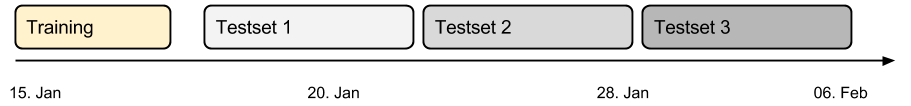
\includegraphics[width=0.24\textwidth]{./time_models/OfflineModel.png}\\
\textbf{\large Bruteforce}\\
On the other hand On-line Learning will change the model with the arriving of new data points.
The bruteforce approach updates the model after a period of time through retraining. Based on a sliding window over the stream with a constant number of data points
the model is rebuilt. The window size for the bruteforce model contains as well 600 data points. After 1000 test points we retrained it with the last 600 data points arrived. We then waited for 1000 data points and second retrain phase with the same window size followed which was tested also with 1000 new data points.\\
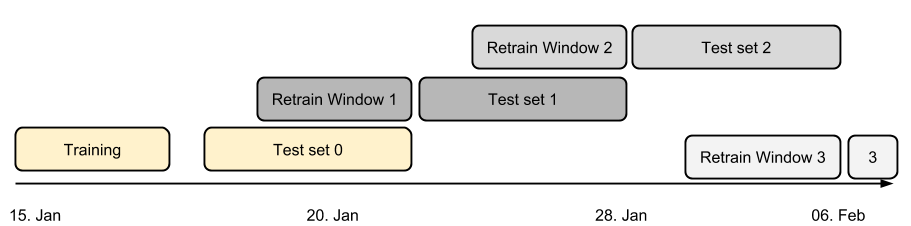
\includegraphics[width=0.2\textwidth]{./time_models/BruteforceModel}\\
\textbf{\large Threshold-triggered}\\
As a variation of the bruteforce model-update, the threshold triggered one will rebuild the model on a sliding window as soon as the accuracy of the model goes below a certain threshold. The window size of the error-triggered model consists of  600 datapoint like in the previous models. We set the accuracy threshold at 63\% which seemed to be a reasonable choice. Sanity window of test points ensures that at least 300 new data points arrive before prematurely throwing out the rebuilt model.\\
\\
\\
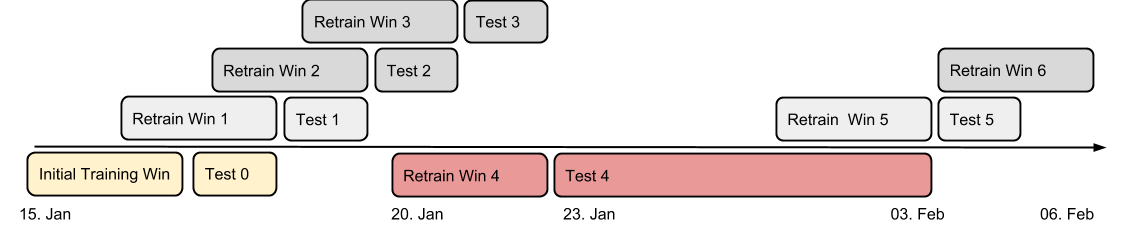
\includegraphics[width=0.2\textwidth]{./time_models/Errortriggered}\\
\textbf{\large Incremental}\\
In the incremental model, unlike the other update models, following an initial training-only phase, all the incoming stream items are always used for training right after the prediction. So, this way the immediate information whether the prediction was good or bad can be used for improving the model on the fly. In other words, predictive model building and testing phases perfectly overlap in incremental model update method. We used this to achieve a real-time response to the changes in the data arguably making the text mining application more resilient to the conceptual drifts. The initial trading size of 600 is used for this model update method as well.

